\chapter{Clases y objetos}

En este punto ya sabes cómo usar funciones para organizar código y tipos integrados para organizar datos. El siguiente paso es aprender ``programación orientada a objetos'', que utiliza tipos definidos por el programador para organizar tanto código como datos. La programación orientada a objetos es un tema extenso; tomará algunos capítulos llegar a dominarlo.

Los ejemplos de código de este capítulo están disponibles en \url{https://thinkpython.com/code/Point1.py}; las soluciones a los ejercicios están disponibles en \url{https://thinkpython.com/code/Point1_soln.py}.

\section{Tipos definidos por el programador}

Hemos usado muchos de los tipos integrados de Python; ahora vamos a definir un nuevo tipo. Como ejemplo, crearemos un tipo llamado \texttt{Point} que representa un punto en el espacio bidimensional.

En notación matemática, los puntos a menudo se escriben entre paréntesis con una coma separando las coordenadas. Por ejemplo, $(0,0)$ representa el origen, y $(x,y)$ representa el punto $x$ unidades a la derecha y $y$ unidades hacia arriba desde el origen.

Hay varias formas en que podríamos representar puntos en Python:

\begin{itemize}
    \item Podríamos almacenar las coordenadas por separado en dos variables, $x$ y $y$.
    \item Podríamos almacenar las coordenadas como elementos en una lista o tupla.
    \item Podríamos crear un nuevo tipo para representar puntos como objetos.
\end{itemize}

Crear un nuevo tipo es más complicado que las otras opciones, pero tiene ventajas que pronto serán evidentes.

Un tipo definido por el programador también se llama \textbf{clase}. Una definición de clase se ve así:

\begin{lstlisting}[language=Python]
class Point:
    """Representa un punto en el espacio 2-D."""
\end{lstlisting}

\begin{figure}[h]
\centering
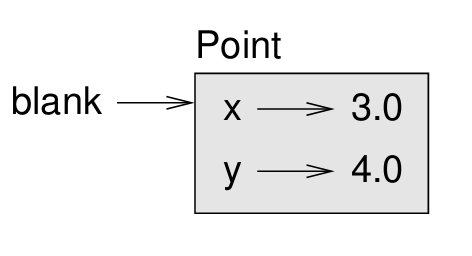
\includegraphics[width=0.7\linewidth]{images/chapter_15_1.png} % Ajusta el nombre del archivo
\caption{Diagrama de objeto.}
\label{fig:diagrama_estado}
\end{figure}

La cabecera indica que la nueva clase se llama \texttt{Point}. El cuerpo es un docstring que explica para qué sirve la clase. Puedes definir variables y métodos dentro de una definición de clase, pero volveremos a eso más adelante.

Definir una clase llamada \texttt{Point} crea un objeto de clase.

\begin{lstlisting}[language=Python]
>>> Point
<class '__main__.Point'>
\end{lstlisting}

Como \texttt{Point} se define en el nivel superior, su ``nombre completo'' es \texttt{\_\_main\_\_.Point}.

El objeto de clase es como una fábrica para crear objetos. Para crear un \texttt{Point}, llamas a \texttt{Point} como si fuera una función.

\begin{lstlisting}[language=Python]
>>> blank = Point()
>>> blank
<__main__.Point object at 0xb7e9d3ac>
\end{lstlisting}

El valor de retorno es una referencia a un objeto \texttt{Point}, que asignamos a \texttt{blank}.

Crear un nuevo objeto se llama \textbf{instanciación}, y el objeto es una \textbf{instancia} de la clase.

Cuando imprimes una instancia, Python te dice a qué clase pertenece y dónde está almacenada en memoria (el prefijo \texttt{0x} significa que el siguiente número está en hexadecimal).

Cada objeto es una instancia de alguna clase, por lo que ``objeto'' e ``instancia'' son intercambiables. Pero en este capítulo usaré ``instancia'' para indicar que estoy hablando de un tipo definido por el programador.

\section{Atributos}

Puedes asignar valores a una instancia usando notación de punto:

\begin{lstlisting}[language=Python]
>>> blank.x = 3.0
>>> blank.y = 4.0
\end{lstlisting}

Esta sintaxis es similar a la sintaxis para seleccionar una variable de un módulo, como \texttt{math.pi} o \texttt{string.whitespace}. En este caso, sin embargo, estamos asignando valores a elementos nombrados de un objeto. Estos elementos se llaman \textbf{atributos}.

Como sustantivo, ``atributo'' se pronuncia con énfasis en la primera sílaba, a diferencia de ``atribuir'', que es un verbo.

La Figura 15.1 es un diagrama de estado que muestra el resultado de estas asignaciones. Un diagrama de estado que muestra un objeto y sus atributos se llama \textbf{diagrama de objetos}.

La variable \texttt{blank} se refiere a un objeto \texttt{Point}, que contiene dos atributos. Cada atributo se refiere a un número de punto flotante.

Puedes leer el valor de un atributo usando la misma sintaxis:

\begin{lstlisting}[language=Python]
>>> blank.y
4.0
>>> x = blank.x
>>> x
3.0
\end{lstlisting}

La expresión \texttt{blank.x} significa: ``Ve al objeto al que \texttt{blank} se refiere y obtén el valor de \texttt{x}''. En el ejemplo, asignamos ese valor a una variable llamada \texttt{x}. No hay conflicto entre la variable \texttt{x} y el atributo \texttt{x}.

Puedes usar notación de punto como parte de cualquier expresión. Por ejemplo:

\begin{lstlisting}[language=Python]
>>> '(%g, %g)' % (blank.x, blank.y)
'(3.0, 4.0)'
>>> distance = math.sqrt(blank.x**2 + blank.y**2)
>>> distance
5.0
\end{lstlisting}

Puedes pasar una instancia como argumento de la manera habitual. Por ejemplo:

\begin{lstlisting}[language=Python]
def print_point(p):
    print('(%g, %g)' % (p.x, p.y))
\end{lstlisting}

\texttt{print\_point} toma un punto como argumento y lo muestra en notación matemática. Para invocarlo, puedes pasar \texttt{blank} como argumento:

\begin{lstlisting}[language=Python]
>>> print_point(blank)
(3.0, 4.0)
\end{lstlisting}

Dentro de la función, \texttt{p} es un alias para \texttt{blank}, por lo que si la función modifica \texttt{p}, \texttt{blank} cambia.

Como ejercicio, escribe una función llamada \texttt{distance\_between\_points} que tome dos \texttt{Points} como argumentos y devuelva la distancia entre ellos.

\section{Rectángulos}

A veces es obvio cuáles deberían ser los atributos de un objeto, pero otras veces tienes que tomar decisiones. Por ejemplo, imagina que estás diseñando una clase para representar rectángulos. ¿Qué atributos usarías para especificar la ubicación y el tamaño del rectángulo? Puedes ignorar el ángulo; para simplificar, asume que el rectángulo es vertical u horizontal.

Hay al menos dos posibilidades:

\begin{itemize}
    \item Podrías especificar una esquina del rectángulo (o el centro), el ancho y la altura.
    \item Podrías especificar dos esquinas opuestas.
\end{itemize}

En este punto es difícil decir si una es mejor que la otra, así que implementaremos la primera, solo como ejemplo.

Aquí está la definición de la clase:

\begin{figure}[h]
\centering
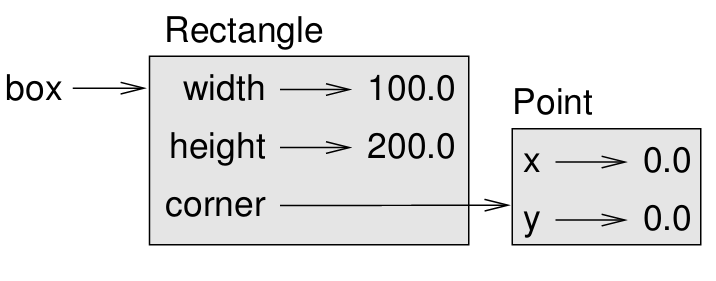
\includegraphics[width=0.7\linewidth]{images/chapter_15_2.png} % Ajusta el nombre del archivo
\caption{Diagrama de objeto.}
\label{fig:diagrama_estado}
\end{figure}

\begin{lstlisting}[language=Python]
class Rectangle:
    """Representa un rectángulo.
    
    atributos: width, height, corner.
    """
\end{lstlisting}

El docstring enumera los atributos: \texttt{width} y \texttt{height} son números; \texttt{corner} es un objeto \texttt{Point} que especifica la esquina inferior izquierda.

Para representar un rectángulo, debes instanciar un objeto \texttt{Rectangle} y asignar valores a los atributos:

\begin{lstlisting}[language=Python]
box = Rectangle()
box.width = 100.0
box.height = 200.0
box.corner = Point()
box.corner.x = 0.0
box.corner.y = 0.0
\end{lstlisting}

La expresión \texttt{box.corner.x} significa: ``Ve al objeto al que \texttt{box} se refiere y selecciona el atributo llamado \texttt{corner}; luego ve a ese objeto y selecciona el atributo llamado \texttt{x}''.

La Figura 15.2 muestra el estado de este objeto. Un objeto que es un atributo de otro objeto está \textbf{incrustado}.

\section{Instancias como valores de retorno}

Las funciones pueden devolver instancias. Por ejemplo, \texttt{find\_center} toma un \texttt{Rectangle} como argumento y devuelve un \texttt{Point} que contiene las coordenadas del centro del \texttt{Rectangle}:

\begin{lstlisting}[language=Python]
def find_center(rect):
    p = Point()
    p.x = rect.corner.x + rect.width/2
    p.y = rect.corner.y + rect.height/2
    return p
\end{lstlisting}

Aquí hay un ejemplo que pasa \texttt{box} como argumento y asigna el \texttt{Point} resultante a \texttt{center}:

\begin{lstlisting}[language=Python]
>>> center = find_center(box)
>>> print_point(center)
(50, 100)
\end{lstlisting}

\section{Los objetos son mutables}

Puedes cambiar el estado de un objeto haciendo una asignación a uno de sus atributos. Por ejemplo, para cambiar el tamaño de un rectángulo sin cambiar su posición, puedes modificar los valores de \texttt{width} y \texttt{height}:

\begin{lstlisting}[language=Python]
box.width = box.width + 50
box.height = box.height + 100
\end{lstlisting}

También puedes escribir funciones que modifiquen objetos. Por ejemplo, \texttt{grow\_rectangle} toma un objeto \texttt{Rectangle} y dos números, \texttt{dwidth} y \texttt{dheight}, y suma los números al ancho y altura del rectángulo:

\begin{lstlisting}[language=Python]
def grow_rectangle(rect, dwidth, dheight):
    rect.width += dwidth
    rect.height += dheight
\end{lstlisting}

Aquí hay un ejemplo que demuestra el efecto:

\begin{lstlisting}[language=Python]
>>> box.width, box.height
(150.0, 300.0)
>>> grow_rectangle(box, 50, 100)
>>> box.width, box.height
(200.0, 400.0)
\end{lstlisting}

Dentro de la función, \texttt{rect} es un alias para \texttt{box}, por lo que cuando la función modifica \texttt{rect}, \texttt{box} cambia.

Como ejercicio, escribe una función llamada \texttt{move\_rectangle} que tome un \texttt{Rectangle} y dos números llamados \texttt{dx} y \texttt{dy}. Debe cambiar la ubicación del rectángulo sumando \texttt{dx} a la coordenada \texttt{x} de \texttt{corner} y sumando \texttt{dy} a la coordenada \texttt{y} de \texttt{corner}.

\section{Copiado}

El uso de alias puede hacer que un programa sea difícil de leer porque los cambios en un lugar pueden tener efectos inesperados en otro lugar. Es difícil hacer un seguimiento de todas las variables que podrían referirse a un objeto dado.

Copiar un objeto es a menudo una alternativa al uso de alias. El módulo \texttt{copy} contiene una función llamada \texttt{copy} que puede duplicar cualquier objeto:

\begin{lstlisting}[language=Python]
>>> p1 = Point()
>>> p1.x = 3.0
>>> p1.y = 4.0

>>> import copy
>>> p2 = copy.copy(p1)
\end{lstlisting}

\texttt{p1} y \texttt{p2} contienen los mismos datos, pero no son el mismo \texttt{Point}.

\begin{lstlisting}[language=Python]
>>> print_point(p1)
(3, 4)
>>> print_point(p2)
(3, 4)
>>> p1 is p2
False
>>> p1 == p2
False
\end{lstlisting}

\begin{figure}[h]
\centering
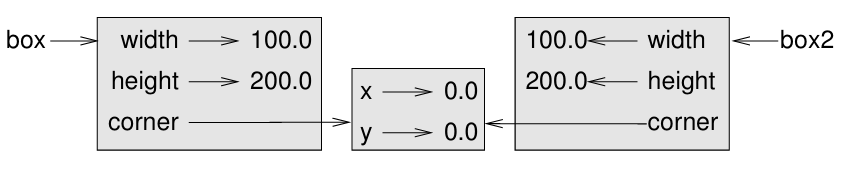
\includegraphics[width=0.7\linewidth]{images/chapter_15_3.png} % Ajusta el nombre del archivo
\caption{Diagrama de onjeto.}
\label{fig:diagrama_estado}
\end{figure}

\begin{lstlisting}
>>> p1 == p2
False
\end{lstlisting}
El operador \texttt{is} indica que \texttt{p1} y \texttt{p2} no son el mismo objeto, que es lo que esperábamos. Pero podrías haber esperado que \texttt{==} devolviera \texttt{True} porque estos puntos contienen los mismos datos. En ese caso, te decepcionará saber que para instancias, el comportamiento predeterminado del operador \texttt{==} es el mismo que el operador \texttt{is}; verifica la identidad del objeto, no la equivalencia del objeto. Esto se debe a que, para tipos definidos por el programador, Python no sabe qué debería considerarse equivalente. Al menos, no todavía.

Si usas \texttt{copy.copy} para duplicar un \texttt{Rectangle}, encontrarás que copia el objeto \texttt{Rectangle} pero no el \texttt{Point} incrustado.

\begin{lstlisting}[language=Python]
>>> box2 = copy.copy(box)
>>> box2 is box
False
>>> box2.corner is box.corner
True
\end{lstlisting}

La Figura 15.3 muestra cómo se ve el diagrama de objetos. Esta operación se llama \textbf{copia superficial} porque copia el objeto y cualquier referencia que contenga, pero no los objetos incrustados.

Para la mayoría de las aplicaciones, esto no es lo que deseas. En este ejemplo, invocar \texttt{grow\_rectangle} en uno de los \texttt{Rectangles} no afectaría al otro, pero invocar \texttt{move\_rectangle} en cualquiera de ellos afectaría a ambos. Este comportamiento es confuso y propenso a errores.

Afortunadamente, el módulo \texttt{copy} proporciona un método llamado \texttt{deepcopy} que copia no solo el objeto sino también los objetos a los que se refiere, y los objetos a los que ellos se refieren, y así sucesivamente. No te sorprenderá saber que esta operación se llama \textbf{copia profunda}.

\begin{lstlisting}[language=Python]
>>> box3 = copy.deepcopy(box)
>>> box3 is box
False
>>> box3.corner is box.corner
False
\end{lstlisting}

\texttt{box3} y \texttt{box} son objetos completamente separados.

Como ejercicio, escribe una versión de \texttt{move\_rectangle} que cree y devuelva un nuevo \texttt{Rectangle} en lugar de modificar el antiguo.

\section{Depuración}

Cuando comienzas a trabajar con objetos, es probable que encuentres algunas excepciones nuevas. Si intentas acceder a un atributo que no existe, obtienes un \texttt{AttributeError}:

\begin{lstlisting}[language=Python]
>>> p = Point()
>>> p.x = 3
>>> p.y = 4
>>> p.z
AttributeError: Point instance has no attribute 'z'
\end{lstlisting}

Si no estás seguro de qué tipo es un objeto, puedes preguntar:

\begin{lstlisting}[language=Python]
>>> type(p)
<class '__main__.Point'>
\end{lstlisting}

También puedes usar \texttt{isinstance} para verificar si un objeto es una instancia de una clase:

\begin{lstlisting}[language=Python]
>>> isinstance(p, Point)
True
\end{lstlisting}

Si no estás seguro de si un objeto tiene un atributo particular, puedes usar la función incorporada \texttt{hasattr}:

\begin{lstlisting}[language=Python]
>>> hasattr(p, 'x')
True
>>> hasattr(p, 'z')
False
\end{lstlisting}

El primer argumento puede ser cualquier objeto; el segundo argumento es una cadena que contiene el nombre del atributo.

También puedes usar una sentencia \texttt{try} para ver si el objeto tiene los atributos que necesitas:

\begin{lstlisting}[language=Python]
try:
    x = p.x
except AttributeError:
    x = 0
\end{lstlisting}

Este enfoque puede facilitar la escritura de funciones que trabajan con diferentes tipos; más sobre ese tema en la Sección 17.9.

\section{Glosario}

\begin{description}
    \item[clase:] Un tipo definido por el programador. Una definición de clase crea un nuevo objeto de clase.
    \item[objeto de clase:] Un objeto que contiene información sobre un tipo definido por el programador. El objeto de clase se puede usar para crear instancias del tipo.
    \item[instancia:] Un objeto que pertenece a una clase.
    \item[instanciar:] Crear un nuevo objeto.
    \item[atributo:] Uno de los valores nombrados asociados con un objeto.
    \item[objeto incrustado:] Un objeto que se almacena como atributo de otro objeto.
    \item[copia superficial:] Copiar el contenido de un objeto, incluidas las referencias a objetos incrustados; implementado por la función \texttt{copy} en el módulo \texttt{copy}.
    \item[copia profunda:] Copiar el contenido de un objeto así como cualquier objeto incrustado, y cualquier objeto incrustado en ellos, y así sucesivamente; implementado por la función \texttt{deepcopy} en el módulo \texttt{copy}.
    \item[diagrama de objetos:] Un diagrama que muestra objetos, sus atributos y los valores de los atributos.
\end{description}

\section{Ejercicios}

\textbf{Ejercicio 15.1.} Escribe una definición para una clase llamada \texttt{Circle} con atributos \texttt{center} y \texttt{radius}, donde \texttt{center} es un objeto \texttt{Point} y \texttt{radius} es un número.

Instancia un objeto \texttt{Circle} que represente un círculo con su centro en $(150,100)$ y radio 75.

Escribe una función llamada \texttt{point\_in\_circle} que tome un \texttt{Circle} y un \texttt{Point} y devuelva \texttt{True} si el \texttt{Point} está dentro o en el límite del círculo.

Escribe una función llamada \texttt{rect\_in\_circle} que tome un \texttt{Circle} y un \texttt{Rectangle} y devuelva \texttt{True} si el \texttt{Rectangle} está completamente dentro o en el límite del círculo.

Escribe una función llamada \texttt{rect\_circle\_overlap} que tome un \texttt{Circle} y un \texttt{Rectangle} y devuelva \texttt{True} si alguna de las esquinas del \texttt{Rectangle} cae dentro del círculo. O como una versión más desafiante, devuelve \texttt{True} si cualquier parte del \texttt{Rectangle} cae dentro del círculo.

Solución: \url{https://thinkpython.com/code/Circle.py}.

\textbf{Ejercicio 15.2.} Escribe una función llamada \texttt{draw\_rect} que tome un objeto \texttt{Turtle} y un \texttt{Rectangle} y use la \texttt{Turtle} para dibujar el \texttt{Rectangle}. Consulta el Capítulo 4 para ver ejemplos de uso de objetos \texttt{Turtle}.

Escribe una función llamada \texttt{draw\_circle} que tome una \texttt{Turtle} y un \texttt{Circle} y dibuje el \texttt{Circle}.

Solución: \url{https://thinkpython.com/code/draw.py}.